\section{Anforderungen und Herausforderungen}
\sectionmark{Anf} % short form for headlines on pages
% Gedankengang beschreiben
% Wie sind wir zur Lösung gekommen?
% Herausforderungen und Probleme nennen
Die Implementierung eines zuverlässigen Parkmanövers stellte den Duckiebot vor mehrere spezifische Anforderungen und Herausforderungen. Zentral war die Fähigkeit, Parklücken visuell zu erkennen und deren Belegung zu bewerten, um nur in freie Slots einzuparken. Dies umfasste die Unterscheidung zwischen freien (\texttt{freeSlot}) und belegten (\texttt{occupiedSlot}) Parkplätzen, die durch spezielle Markierungen in der Duckietown-Umgebung definiert sind. Die Wahrnehmung erfolgte hierbei primär durch die bereits in Challenge 3 (Kapitel~\ref{ch:Challenge_3}) etablierte Objekterkennungs-Pipeline, welche die notwendigen Bounding Boxes lieferte.

Eine wesentliche Herausforderung war die präzise Lokalisierung der Parklücke und die Ableitung einer geeigneten Zielposition für das rückwärtige Einparken. Dies erforderte eine robuste Bildverarbeitung, die unabhängig von wechselnden Lichtverhältnissen und Perspektiven die gelben Begrenzungslinien der Parklücke zuverlässig detektieren konnte. Besondere Schwierigkeiten ergaben sich aus der Notwendigkeit, das Fahrzeug exakt rückwärts in die Lücke zu manövrieren, da dies ein hohes Maß an Steuerungsgenauigkeit und Stabilität der Rückkopplungsschleife erforderte. Herkömmliche Spurhaltungsalgorithmen sind typischerweise für die Vorwärtsfahrt optimiert und mussten für dieses Szenario angepasst oder ergänzt werden.

Des Weiteren musste sichergestellt werden, dass das Parkmanöver als hochpriorisierter Prozess abläuft und nicht durch konkurrierende Steuerbefehle (z.B. der allgemeinen Spurverfolgung oder der Kollisionsvermeidung durch den \ac{ToF}-Sensor, sofern aktiv) gestört oder abgebrochen wird. Die Zustandsübergänge des Parkvorgangs – von der Annäherung über das Einparken bis zum Warten und Ausparken – mussten klar definiert und zeitlich kontrolliert werden, um ein flüssiges und regelkonformes Verhalten zu gewährleisten. Dazu gehörte auch die sichere Detektion des \enquote{eingeparkten} Zustands und die anschließende Wiederaufnahme der Fahrt nach einer definierten Wartezeit.

\newpage

Schließlich war die Integration von visuellen Rückmeldungen (Blinkern) während des Manövers eine zusätzliche Anforderung, um die Interaktion des Duckiebots mit der Umgebung transparenter zu gestalten. Dies erforderte die Ansteuerung der LED-Elemente des Roboters in Abhängigkeit vom aktuellen Parkstatus.

\section{Ablaufdiagramm}
\sectionmark{Impl} % short form for headlines on pages
% Ablaufdiagramm und Beschreibung der Node
Das Parkmanöver des Duckiebots wird durch eine mehrstufige Zustandsmaschine in der \texttt{parking\_node} gesteuert, deren Ablauf in Abbildung~\ref{fig:parking_flow} dargestellt ist.

\begin{figure}[htbp]
    \centering
    % Erster Teil des Diagramms
    \begin{minipage}[c]{0.5\textwidth} % oder eine andere Breite, je nach Bedarf
        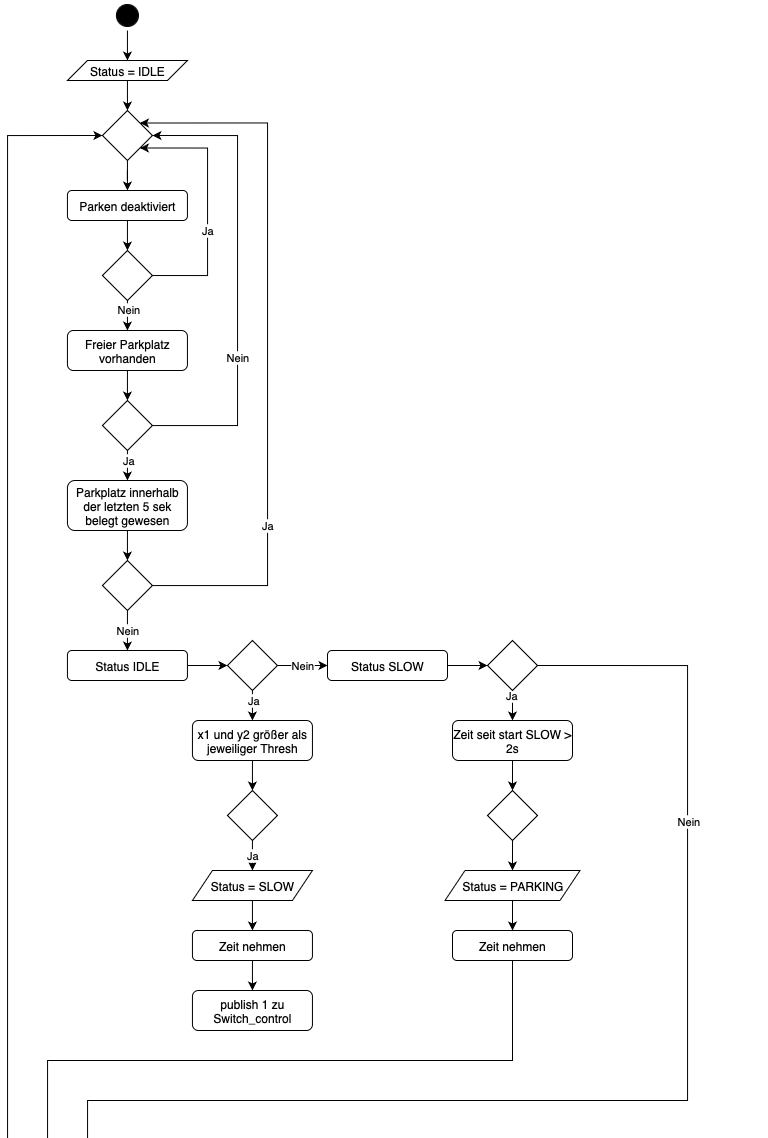
\includegraphics[width=\linewidth]{Figures/png/Ablaufdiagramm_Parken_1.png}
        % Optional: Eine Unterbeschriftung für diesen Teil, falls nötig
        %\caption*{Teil 1} 
    \end{minipage}%
    \hfill % Optionaler Platz zwischen den Minipages
    % Zweiter Teil des Diagramms
    \begin{minipage}[c]{0.5\textwidth} % oder eine andere Breite
        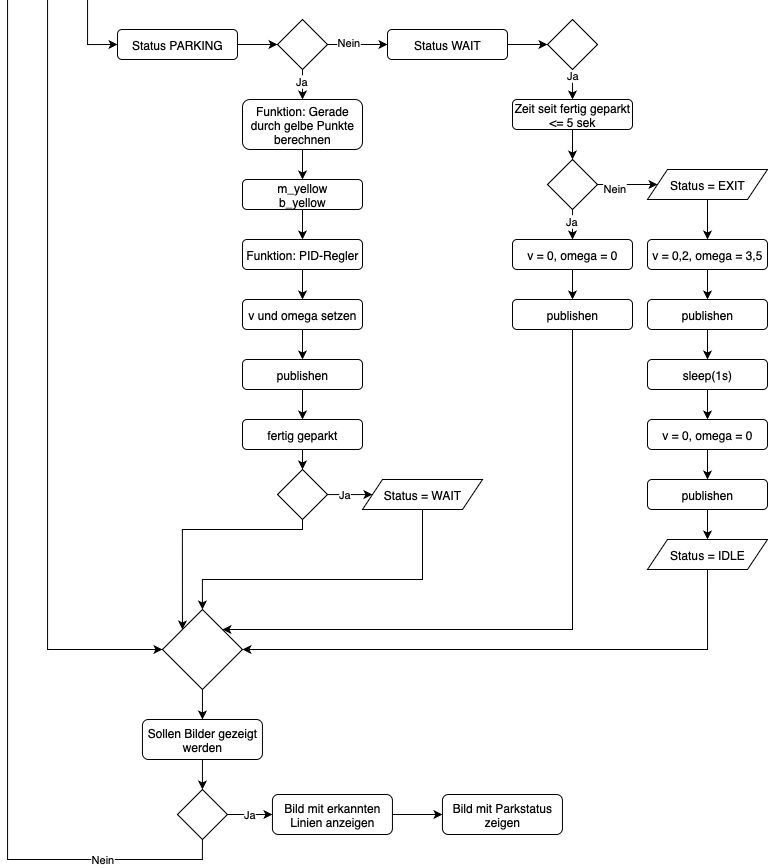
\includegraphics[width=\linewidth]{Figures/png/Ablaufdiagramm_Parken_2.png}
        % Optional: Eine Unterbeschriftung für diesen Teil, falls nötig
        %\caption*{Teil 2}
    \end{minipage}
    \caption{Ablaufdiagramm der Parking Node}
    \label{fig:parking_flow}
\end{figure}

Der Prozess beginnt im Zustand \texttt{IDLE}, in dem der Duckiebot die Umgebung kontinuierlich nach einer freien Parklücke überwacht. Sobald eine freie Parklücke durch die \texttt{detect\_object\_node} erkannt und deren Bounding Box eine vordefinierte Position im Kamerabild erreicht (d.h., die Lücke ist direkt vor dem Bot und im richtigen Winkel), wechselt das System in den Zustand \texttt{SLOW}.

Im \texttt{SLOW}-Zustand reduziert der Duckiebot seine Geschwindigkeit und nähert sich der Parklücke an. Dieser Zustand dient einer kontrollierten Vorbereitung des eigentlichen Parkvorgangs und dauert zwei Sekunden, um dem System Zeit für die Stabilisierung der Wahrnehmung zu geben. Während dieser Phase wird zudem ein gelbes Blinksignal aktiviert, um das bevorstehende Manöver anzuzeigen.

Nach Ablauf der Wartezeit erfolgt der Übergang in den Zustand \texttt{PARKING}. Hier beginnt das rückwärtige Einparkmanöver. Die \texttt{parking\_node} nutzt eine eigene Implementierung zur Erkennung der gelben Parklinien im unteren Bereich des Bildes und steuert den Duckiebot mittels eines PID-Reglers, um die gelbe Linie auf eine feste Ziel-Y-Koordinate auszurichten. Die Geschwindigkeit ist dabei negativ, um die Rückwärtsfahrt zu ermöglichen. Das System verbleibt in diesem Zustand, bis die lateralen und Winkelabweichungen zur Ziellinie gering genug sind oder die gelbe Linie hinter der Ziellinie liegt, was das erfolgreiche Einparken signalisiert.

Wurde das Fahrzeug erfolgreich eingeparkt, wechselt es in den Zustand \texttt{WAIT}. In diesem Zustand verweilt der Duckiebot für fünf Sekunden im Stillstand, um eine temporäre Parkdauer oder einen Ladestopp zu simulieren. Das Blinksignal wird währenddessen deaktiviert.

Nach Ablauf der Wartezeit geht der Duckiebot in den Zustand \texttt{EXIT} über. Hier führt er ein kurzes Ausfahrmanöver aus (fest definierte Vorwärts- und Lenkbefehle für eine Sekunde), um die Parklücke zu verlassen. Auch hier wird wieder ein Blinksignal aktiviert.

Nachdem das Ausfahren abgeschlossen ist, stoppt der Duckiebot kurz und kehrt in den \texttt{IDLE}-Zustand zurück, um die normale Spurverfolgung oder andere Fahrfunktionen wieder aufzunehmen und auf die nächste Parklücke oder andere Anweisungen zu warten.




\section{Technische Umsetzung im Code}
\sectionmark{Tech} % short form for headlines on pages
% Beschreibung wie man es im Code umgesetzt hat
Die technische Realisierung des Parkmanövers erfolgt hauptsächlich durch die \texttt{parking\_node}, die die Erkennung von Parklücken, die Zustandslogik des Parkvorgangs und die Steuerung des Duckiebots während des Manövers koordiniert. Sie interagiert dabei mit anderen Systemkomponenten, insbesondere der Objekterkennungs-Node und der \texttt{car\_cmd\_switch\_node}.


\subsection{Parklückenerkennung und -auswahl}
Die \texttt{parking\_node} abonniert die \ac{ROS}-Topics \texttt{/detect/object/parkingBB} und \texttt{/detect/object/parkingOccupiedBB}, die von der \texttt{detect\_object\_node} (wie in Kapitel~\ref{ch:Challenge_2} beschrieben) mit Bounding Boxes erkannter Parklücken beliefert werden. Diese Bounding Boxes enthalten die visuellen Koordinaten der Parklücken im Kamerabild. Die \texttt{parking\_node} entscheidet basierend auf der veröffentlichten Klassifizierung (\enquote{free} oder \enquote{occupied}) und der zeitlichen Gültigkeit (time\_lastFree, time\_lastOccupied) über die Eignung eines Parkplatzes. Ein Parkvorgang wird nur eingeleitet, wenn eine freie Parklücke erkannt wird und sich diese in einem definierten Bereich des Kamerabildes befindet (durch die Parameter \texttt{xForSlowDrive} und \texttt{yForSlowDrive} in der YAML-Konfiguration festgelegt).

\newpage


\subsection{Zustandsmanagement und Manövrierung}
Die Kernlogik ist eine finite Zustandsmaschine mit den Modi IDLE, SLOW, PARKING, WAIT und EXIT. Die Übergänge zwischen diesen Zuständen werden durch Timer und sensorische Rückmeldungen gesteuert:
\begin{itemize}
\item \textbf{\texttt{IDLE} $\rightarrow$ \texttt{SLOW}:} Eine freie Parklücke wird im definierten Bereich der Kamerabildes erkannt.
\item \textbf{\texttt{SLOW} $\rightarrow$ \texttt{PARKING}:} Nach einer 2-sekündigen Annäherungsphase, in der die Geschwindigkeit des Duckiebots reduziert wird.
\item \textbf{\texttt{PARKING} $\rightarrow$ \texttt{WAIT}:} Sobald der Duckiebot erfolgreich rückwärts in die Parklücke manövriert wurde. Der Erfolg wird durch einen geringen lateralen und Winkel-Fehler der gelben Parklinien zur Zielgeraden (\texttt{self.m\_target}, \texttt{self.b\_target}) signalisiert.
\item \textbf{\texttt{WAIT} $\rightarrow$ \texttt{EXIT}:} Nach einer Wartezeit von 5 Sekunden im geparkten Zustand.
\item \textbf{\texttt{EXIT} $\rightarrow$ \texttt{IDLE}:} Nach einer 1-sekündigen Ausfahrbewegung, um die Parklücke zu verlassen.
\end{itemize}

Während des \texttt{PARKING}-Zustands kommt eine spezifische bildbasierte Regelung zum Einsatz. Die Funktion \texttt{detect\_yellow} identifiziert die gelbe Parklinien im Kamerabild (unter Verwendung von \ac{HSV}-Farbraummasken, morphologischen Operationen und Konturerkennung, ähnlich der Spurverfolgung). Aus diesen detektierten Linien wird eine geglättete Linie abgeleitet (\texttt{m\_yellow\_smooth}, \texttt{b\_yellow\_smooth}). Die Funktion \texttt{calculate\_control} berechnet dann basierend auf einem PID-Regler die notwendigen Lenk- (\texttt{omega}) und Geschwindigkeitsbefehle (\texttt{v}). Der Fehler für den PID-Regler wird aus der Abweichung der erkannten gelben Linie von einer definierten Zielgeraden im Bild ($y=270$) ermittelt. Der Duckiebot fährt dabei rückwärts (negativer \texttt{v}-Wert), um sich an der gelben Linie auszurichten und präzise in die Lücke einzufahren. Die Glättung von Linienparametern und Fehlern über Historien (\texttt{smooth\_N}, \texttt{smooth\_error\_N}) sorgt für ein ruhigeres Fahrverhalten.

Die Kommunikation mit der zentralen Steuerung (\texttt{switch\_control\_node}) erfolgt über das Topic \texttt{/detect/object/slow4park}. Die \texttt{parking\_node} publiziert hier einen Statuscode (\texttt{Int32(5)} für \texttt{PARKING}, \texttt{WAIT}, \texttt{EXIT}; \texttt{1} für \texttt{SLOW}). Dadurch wird der \texttt{switch\_control\_node} signalisiert, die Steuerungspriorität für den Parkvorgang zu erhöhen oder eine reduzierte Geschwindigkeit für die Annäherung beizubehalten, während andere Funktionen (wie die Spurverfolgung) temporär unterdrückt werden.


\subsection{Visuelle Rückmeldung (Blinker)}
Zur visuellen Anzeige des Parkmanövers werden die LEDs des Duckiebots als Blinker aktiviert. Beim Übergang in den \texttt{SLOW}- und \texttt{EXIT}-Zustand wird ein gelbes Blinkmuster mit einer Frequenz von 2\,Hz auf den vorderen und hinteren seitlichen LEDs aktiviert. Dies erfolgt über eine \ac{ROS}-Timer-Funktion (\texttt{blink\_all\_leds}), die die LED-Muster auf dem Topic \texttt{/led\_emitter\_node/led\_pattern} publiziert. Während des \texttt{WAIT}-Zustands sind die LEDs ausgeschaltet, und nach Abschluss des Parkvorgangs (Rückkehr zu \texttt{IDLE}) werden die LEDs wieder in den Standardzustand zurückgesetzt.

\newpage

\subsection{Zusammenfassung}
Die \texttt{parking\_node} bietet eine umfassende Lösung für autonome Parkmanöver, die auf einer robusten Kombination aus Parklückenerkennung, einer flexiblen Zustandsmaschine und einer präzisen PID-basierten Rückwärtslenkung basiert. Die Integration mit dem übergeordneten Steuerungssystem des Duckiebots gewährleistet eine nahtlose Einbindung in das Gesamtsystem, während die visuellen Rückmeldungen die Benutzerinteraktion verbessern.

%% End of File %%